\section{Introducción a los PEGs}

In computer science, a \cei{parsing expression grammar}, or \cei{PEG}, is a type of
analytic formal grammar, i.e. it describes a formal language in terms
of a set of rules for recognizing strings in the language.

The formalism was introduced by 
\htmladdnormallink{Bryan Ford in 2004 }{https://pdos.csail.mit.edu/papers/parsing:popl04.pdf}
and is closely related to the family of top-down parsing languages introduced in the early 1970s. 

Syntactically, PEGs also look similar to
context-free grammars (CFGs), but they have a different interpretation: 

\begin{itemize}
\item
the choice operator selects the first match in PEG, while it is ambiguous in CFG. 
\item
This is closer to how string recognition tends
to be done in practice, e.g. by a recursive descent parser.
\end{itemize}

Unlike CFGs, PEGs cannot be \underline{ambiguous}; 
{\it if a string parses, it has exactly
one valid parse tree}. 

It is conjectured that there exist context-free
languages that cannot be parsed by a PEG, but this is
not yet proven. 

\subsection{Syntax}
Formally, a parsing expression grammar consists of:
\begin{itemize}
\item
A finite set $N$ of nonterminal symbols.
\item
A finite set $\Sigma$ of terminal symbols that is disjoint from $N$.
\item
A finite set $P$ of parsing rules.
\item
An expression $e_S$ termed the starting expression.
\end{itemize}

Each parsing rule in $P$ 
has the form $A \leftarrow e$, 
where $A$ is a nonterminal symbol and $e$ is a \cei{parsing expression}. 

A parsing expression is a hierarchical expression similar to a regular expression, which is
constructed in the following fashion:
\begin{enumerate}
\item
An atomic parsing expression consists of:
\begin{enumerate}
\item any terminal symbol,
\item any nonterminal symbol, or
\item the empty string $\epsilon$.
\end{enumerate}
\item
Given any existing parsing expressions $e$, $e_1$, and $e_2$, 
a new parsing
expression can be constructed using the following operators:
\begin{enumerate}
\item
Sequence: $e1 e2$
\item
Ordered choice: $e1 / e2$
\item
Zero-or-more: $e*$
\item
One-or-more: $e+$
\item
Optional: $e?$
\item
And-predicate: $\&e$
\item
Not-predicate: $!e$
\end{enumerate}
\end{enumerate}

\subsection{Semantics}

The fundamental difference between context-free grammars and parsing
expression grammars is that the PEG's choice operator is {\color{red} ordered}:

\begin{enumerate}
\item
If
the first alternative succeeds, the second alternative is
ignored. 
\item
Thus ordered choice is not commutative, unlike unordered choice as in context-free grammars.
\item
The consequence is that if a CFG is transliterated directly to a PEG,
any ambiguity in the former is resolved by deterministically picking
one parse tree from the possible parses. 
\item
By carefully
choosing the order in which the grammar alternatives are specified, a programmer has a great deal of control over which parse tree is selected.
\item
PEGs can {\color{red} look ahead} into the
input string without actually consuming it
\item
The and-predicate expression $\&e$ invokes the sub-expression $e$, 
and then succeeds if $e$ succeeds and fails if $e$ fails, 
{\it but in either case never consumes any input}.
\item
The not-predicate expression $!e$ succeeds if $e$ 
fails and fails if $e$ succeeds, {\it again consuming no input in either case}.
\end{enumerate}

\subsection{Implementing parsers from parsing expression grammars}

Any parsing expression grammar can be converted directly into a \cei{recursive descent parser}. 

Due to the unlimited lookahead capability that the grammar formalism
provides, however, the resulting parser {\color{red} could exhibit exponential time
performance in the worst case}.

It is possible to obtain better performance for any parsing expression
grammar by converting its recursive descent parser into {\color{red} a 
\htmladdnormallink{packrat parser}{http://bford.info/pub/lang/packrat-icfp02/},
which always runs in linear time}, at the cost of substantially greater
storage space requirements. 

{\it A packrat parser is a form of parser
similar to a recursive descent parser in construction, except that
during the parsing process {\colorbox{black}{\color{Violet} it memoizes}}
the intermediate results of all
invocations of the mutually recursive parsing functions}, ensuring that
each parsing function is only invoked at most once at a given input
position. 

Because of this memoization, a packrat parser has the ability
to parse many context-free grammars and any parsing expression grammar
(including some that do not represent context-free languages) in linear
time. 

Examples of memoized recursive descent parsers are known from at
least as early as 1993. 

Note that this analysis of the performance
of a packrat parser {\bf assumes that enough memory is available to hold all
of the memoized results}; in practice, if there were not enough memory,
some parsing functions might have to be invoked more than once at the
same input position, and consequently the parser could take more than
linear time.

It is also possible to build LL parsers and LR parsers from parsing
expression grammars, with better worst-case performance than a recursive
descent parser, but the unlimited lookahead capability of the grammar
formalism is then lost. Therefore, not all languages that can be expressed
using parsing expression grammars can be parsed by LL or LR parsers.

\subsection{Lexical Analysis}

Parsers for languages expressed as a CFG, such as LR parsers, require a
separate tokenization step to be done first, which breaks up the input
based on the location of spaces, punctuation, etc. 

The tokenization is
necessary because of the way these parsers use lookahead to parse CFGs
that meet certain requirements in linear time. 

PEGs do
not require tokenization to be a separate step, and tokenization rules
can be written in the same way as any other grammar rule.

\subsection{Left recursion}

PEGs cannot express left-recursive rules where a rule refers to itself
without moving forward in the string. 
 For example, the following left-recursive CFG rule:
\begin{verbatim}
string-of-a -> string-of-a 'a' | 'a'
\end{verbatim}
can be rewritten in a PEG using the plus operator:
\begin{verbatim}
string-of-a <- 'a'+
\end{verbatim}
The process of rewriting indirectly left-recursive rules is complex in some packrat parsers, especially when semantic actions are involved.

\subsection{Referencias y Documentación}
\begin{itemize}
\item
Véase \wikip{Parsing Expression Grammar}{Parsing_expression\_grammar}
\item
\htmladdnormallink{PEG.js documentation}{http://pegjs.majda.cz/documentation}
\item
\htmladdnormallink{Testing PEG.js Online}{http://pegjs.majda.cz/online}
\item
Michael's Blog: \htmladdnormallink{JavaScript Parser Generators}{http://blog.mi-ernst.de/2012/05/14/javascript-parser-generators/}.
The PEG.js Tutorial
\item
\htmladdnormallink{The Packrat Parsing and 
Parsing Expression Grammars Page}{http://bford.info/packrat/}
\item
\htmladdnormallink{PL101: Create Your Own Programming Language}{http://nathansuniversity.com/}.
Véanse \cite{nathanuniversity} y 
\cite{nathanclosures}
\item
\htmladdnormallink{PL101: Create Your Own Programming Language: Parsing}{http://nathansuniversity.com/pegs.html}
\end{itemize}

\section{PEGJS}

\parrafo{What is}

\pegjs{} is a parser generator for JavaScript that produces 
parsers. 

\pegjs{} generates a parser from a Parsing Expression Grammar 
describing a language.

We can specify what the parser returns (using semantic actions on matched
parts of the input). 

\parrafo{Installation}

To use the pegjs command, install \pegjs{} globally:

\begin{verbatim}
$ npm install -g pegjs
\end{verbatim}
To use the JavaScript API, install \pegjs{} locally:

\begin{verbatim}
$ npm install pegjs
\end{verbatim}

To use it from the browser, download the 
\pegjs{}
library (
\htmladdnormallink{regular }{https://github.com/dmajda/pegjs/releases/download/v0.8.0/peg-0.8.0.js}
or \htmladdnormallink{minified version}{https://github.com/dmajda/pegjs/releases/download/v0.8.0/peg-0.8.0.min.js}).

\parrafo{El compilador de línea de comandos}

\begin{verbatim}
[~/srcPLgrado/pegjs/examples(master)]$ pegjs --help
Usage: pegjs [options] [--] [<input_file>] [<output_file>]

Generates a parser from the PEG grammar specified in the <input_file> and writes
it to the <output_file>.

If the <output_file> is omitted, its name is generated by changing the
<input_file> extension to ".js". If both <input_file> and <output_file> are
omitted, standard input and output are used.

Options:
  -e, --export-var <variable>        name of the variable where the parser
                                     object will be stored (default:
                                     "module.exports")
      --cache                        make generated parser cache results
      --allowed-start-rules <rules>  comma-separated list of rules the generated
                                     parser will be allowed to start parsing
                                     from (default: the first rule in the
                                     grammar)
  -o, --optimize <goal>              select optimization for speed or size
                                     (default: speed)
      --plugin <plugin>              use a specified plugin (can be specified
                                     multiple times)
      --extra-options <options>      additional options (in JSON format) to pass
                                     to PEG.buildParser
      --extra-options-file <file>    file with additional options (in JSON
                                     format) to pass to PEG.buildParser
  -v, --version                      print version information and exit
  -h, --help                         print help and exit
\end{verbatim}

\parrafo{Using it}

\begin{verbatim}
[~/srcPLgrado/pegjs/examples(master)]$ node
> PEG = require("pegjs")
{ VERSION: '0.8.0',
  GrammarError: [Function],
  parser: 
   { SyntaxError: [Function: SyntaxError],
     parse: [Function: parse] },
  compiler: 
   { passes: 
      { check: [Object],
        transform: [Object],
        generate: [Object] },
     compile: [Function] },
  buildParser: [Function] }
\end{verbatim}
\begin{verbatim}
> parser = PEG.buildParser("start = ('a' / 'b')+")
{ SyntaxError: [Function: SyntaxError],
  parse: [Function: parse] }
\end{verbatim}

Using the generated parser is simple — just call its \verb|parse| method
and pass an input string as a parameter. 

The method will return 
\begin{itemize}
\item
a parse result (the exact value depends on the grammar used to build the parser) or 
\item
throw an \red{exception} if the input is invalid.  

The exception will contain 
\verb|offset|, \verb|line|, \verb|column|, \verb|expected|, \verb|found| and \verb|message| 
properties with more details about the error.
\end{itemize}
You can tweak parser behavior by passing a second parameter with
an \verb|options| object to the \verb|parse| method. 

Only one option is currently supported:

\verb|startRule| which is the name of the rule to start parsing from.



\begin{verbatim}
> parser.parse("abba"); 
[ 'a', 'b', 'b', 'a' ]
> 
\end{verbatim}

\parrafo{Opciones: allowedStartRules}
Specifying
\red{allowedStartRules} we can set the
rules the parser will be allowed to start parsing from (default: the first rule in the grammar).

\begin{verbatim}
[~/srcPLgrado/pegjs/examples(master)]$ cat allowedstartrules.js 
var PEG = require("pegjs");
var grammar = "a = 'hello' b\nb = 'world'"; //"a = 'hello' b\nb='world';
console.log(grammar); // a = 'hello' b
                      // b = 'world'
var parser = PEG.buildParser(grammar,{ allowedStartRules: ['a', 'b'] });
var r = parser.parse("helloworld", { startRule: 'a' });
console.log(r); // [ 'hello', 'world' ]
r = parser.parse("helloworld")
console.log(r); // [ 'hello', 'world' ]

r =  parser.parse("world", { startRule: 'b' })
console.log(r); // 'world'

try {
  r = parser.parse("world"); // Throws an exception
}
catch(e) {
  console.log("Error!!!!");
  console.log(e);
}
\end{verbatim}

\begin{verbatim}
[~/srcPLgrado/pegjs/examples(master)]$ node allowedstartrules.js 
a = 'hello' b
b = 'world'
[ 'hello', 'world' ]
[ 'hello', 'world' ]
world
Error!!!!
{ message: 'Expected "hello" but "w" found.',
  expected: [ { type: 'literal', value: 'hello', description: '"hello"' } ],
  found: 'w',
  offset: 0,
  line: 1,
  column: 1,
  name: 'SyntaxError' }
\end{verbatim}

The \red{exception} contains
\begin{itemize}
\item
message 
\item
expected, 
\item
found 
\item
offset, 
\item
line, 
\item
column, 
\item
name
\end{itemize}
and properties with more details about the error.

\parrafo{Opciones: output}

\begin{itemize}
\item
When
\verb|output|
is set to \red{parser}, the method will return generated parser object; 
\begin{verbatim}
> PEG = require("pegjs")
> grammar = "a = 'hello' b\nb='world'"
'a = \'hello\' b\nb=\'world\''
> console.log(grammar)
a = 'hello' b
b='world'
> parser = PEG.buildParser(grammar,{ output: "parser"})
{ SyntaxError: [Function: SyntaxError],
  parse: [Function: parse] }
  > parser.parse("helloworld")
  [ 'hello', 'world' ]
\end{verbatim}
\item
if set to \blue{source}, it will return parser source code as a string 
\begin{verbatim}
> parser = PEG.buildParser(grammar,{ output: "source"})
> typeof parser
'string'
> console.log(parser.substring(0,100))
(function() {
  /*
   * Generated by PEG.js 0.8.0.
   *
   * http://pegjs.majda.cz/
   */
\end{verbatim}
\item
(default: \verb"parser").
\end{itemize}


\parrafo{Opciones: plugin}
La opción 
\red{plugins}
indica que plugin se van a usar.
\begin{verbatim}
$ pegjs --plugin pegjs-coffee-plugin remove_left_recursive.pegjs 
\end{verbatim}

\parrafo{PEGjs  Coffee Plugin }

\htmladdnormallink{PEGjs Coffee Plugin }{https://github.com/Dignifiedquire/pegjs-coffee-plugin}
is a plugin for PEG.js to use CoffeeScript in actions.

\begin{verbatim}
[~/srcPLgrado/pegjs_examples(master)]$ cat plugin.coffee 
#!/usr/bin/env coffee
PEG = require 'pegjs'
coffee = require 'pegjs-coffee-plugin'
grammar = """
a = 'hello' _ b { console.log 3; "hello world!" }
b = 'world'     { console.log 2 }
_ = [ \t]+      { console.log 1 }
"""
parser = PEG.buildParser grammar, plugins: [coffee]
r = parser.parse "hello world"
console.log("r = #{r}")
\end{verbatim}
La ejecución nos muestra además el orden de abajo - arriba
y de izquierda -derecha en la ejecución de las acciones 
semánticas:
\begin{verbatim}
[~/srcPLgrado/pegjs_examples(master)]$ coffee plugin.coffee 
1
2
3
r = hello world!
\end{verbatim}

\parrafo{Instalación de pegjs-coffee-plugin}
\begin{verbatim}
[~/Dropbox/src/javascript/PLgrado/pegjs/examples(master)]$ npm install -g pegjs-coffee-plugin
\end{verbatim}

\parrafo{Ejemplo con Acciones Semánticas en Coffee}
\begin{verbatim}
[~/Dropbox/src/javascript/PLgrado/pegjs-coffee-plugin/examples(master)]$ cat simple.pegjs 
{ 
  @reduce = (left, right)->  
    sum = left
    for t in right
      op = t[0]
      num = t[1]
      switch op 
        when '+' then sum += num; break
        when '-' then sum -= num; break
        when '*' then sum *= num; break
        when '/' then sum /= num; break
        else console.log("Error! "+op)
    sum
  
}
sum   = left:product right:([+-] product)* { @reduce(left, right); }
product = left:value right:([*/] value)*   { @reduce(left, right); }
value   = number:[0-9]+                    { parseInt(number.join(''),10) }
        / '(' sum:sum ')'                  { sum }
\end{verbatim}

\begin{verbatim}
[~/Dropbox/src/javascript/PLgrado/pegjs-coffee-plugin/examples(master)]$  cat use_simple.coffee 
PEG = require("./simple.js")
r = PEG.parse("2+3*(2+1)-10/2")
console.log(r)
\end{verbatim}


\begin{verbatim}
[~/srcPLgrado/pegjs/examples/coffee-plugin-examples(master)]$ pegjs --plugin pegjs-coffee-plugin simple.pegjs
[~/srcPLgrado/pegjs/examples/coffee-plugin-examples(master)]$ coffee use_simple.coffee
input = 3-1-2 result = 0
input = 2+3*(2+1)-10/2 result = 6
\end{verbatim}


\parrafo{Véase También}
\begin{itemize}
\item
\htmladdnormallink{pegjs-coffee-plugin}{https://github.com/Dignifiedquire/pegjs-coffee-plugin}
en GitHub
\end{itemize}


\parrafo{cache}

If \verb|true|, makes the parser cache results, avoiding exponential parsing
time in pathological cases but making the parser slower (default:
\verb|false|).

\parrafo{optimize}

Selects between optimizing the generated parser for parsing speed
(\verb"speed") or code size (\verb"size") (default: \verb"speed").


\section{Un Ejemplo Sencillo}
\label{section:UnEjemploSencillo}

\parrafo{Donde}
\begin{verbatim}
[~/srcPLgrado/pegjs/examples(master)]$ pwd -P
/Users/casiano/local/src/javascript/PLgrado/pegjs/examples
[~/srcPLgrado/pegjs/examples(master)]$ git remote -v
dmajda  https://github.com/dmajda/pegjs.git (fetch)
dmajda  https://github.com/dmajda/pegjs.git (push)
origin  git@github.com:crguezl/pegjs.git (fetch)
origin  git@github.com:crguezl/pegjs.git (push)
\end{verbatim}

\htmladdnormallink{https://github.com/crguezl/pegjs/blob/master/examples/arithmetics.pegjs}{https://github.com/crguezl/pegjs/blob/master/examples/arithmetics.pegjs}

\parrafo{arithmetics.pegjs}

The grammar syntax is similar to JavaScript in that it is not
line-oriented and ignores whitespace between tokens. 

You can also use
JavaScript-style comments (\verb|// ...| and \verb|/* ... */|).

Let's look at example grammar that recognizes simple arithmetic
expressions like \verb|2*(3+4)|. 

A parser generated from this grammar computes
their values.

\begin{verbatim}
[~/Dropbox/src/javascript/PLgrado/pegjs/examples(master)]$ cat arithmetics.pegjs 
/*
 * Classic example grammar, which recognizes simple arithmetic expressions like
 * "2*(3+4)". The parser generated from this grammar then computes their value.
 */

start
  = additive

additive
  = left:multiplicative PLUS right:additive { return left + right; }
  / left:multiplicative MINUS right:additive { return left - right; }
  / multiplicative

multiplicative
  = left:primary MULT right:multiplicative { return left * right; }
  / left:primary DIV right:multiplicative { return left / right; }
  / primary

primary
  = integer
  / LEFTPAR additive:additive RIGHTPAR { return additive; }

integer "integer"
  = NUMBER

_ = $[ \t\n\r]*

PLUS = _"+"_
MINUS = _"-"_
MULT = _"*"_
DIV = _"/"_
LEFTPAR = _"("_
RIGHTPAR = _")"_
NUMBER = _ digits:$[0-9]+ _ { return parseInt(digits, 10); }
\end{verbatim}


\parrafo{main.js}

\begin{verbatim}
[~/Dropbox/src/javascript/PLgrado/pegjs/examples(master)]$ cat main.js 
var PEG = require("./arithmetics.js");
var r = PEG.parse("(2+9-1)/2");
console.log(r);
\end{verbatim}

\parrafo{Rakefile}

\begin{verbatim}
[~/Dropbox/src/javascript/PLgrado/pegjs/examples(master)]$ cat Rakefile 
PEGJS = "../bin/pegjs"
task :default => :run

desc "Compile arithmetics.pegjs"
task :compile do
  sh "#{PEGJS} arithmetics.pegjs"
end

desc "Run and use the parser generated from arithmetics.pegjs"
task :run => :compile do
  sh "node main.js"
end
\end{verbatim}

\parrafo{Compilación}
\begin{verbatim}
[~/Dropbox/src/javascript/PLgrado/pegjs/examples(master)]$ rake
../bin/pegjs arithmetics.pegjs
node main.js
5
\end{verbatim}

\subsection{Asociación Incorrecta para la Resta y la División}

\begin{definition}
Una \cei{gramática es recursiva por la izquierda} cuando existe una derivación
$A \stackrel{*}{\Longrightarrow} A \alpha$. 

En particular, es recursiva por la izquierda si contiene
una regla de producción de la forma $A \rightarrow A \alpha$. 
En este caso se dice que la recursión por la izquierda es directa.
\end{definition}

Cuando la gramática es \cei{recursiva por la izquierda}, 
el método 
de análisis recursivo descendente predictivo no funciona. 
En ese caso, el procedimiento
\verb|A| asociado con $A$ ciclaría para siempre sin llegar a consumir ningún 
terminal. 

Es por eso que hemos escrito las reglas de la calculadora con recursividad
a derechas, 
\begin{verbatim}
additive
  = left:multiplicative PLUS right:additive { return left + right; }
  / left:multiplicative MINUS right:additive { return left - right; }
  / multiplicative

multiplicative
  = left:primary MULT right:multiplicative { return left * right; }
  / left:primary DIV right:multiplicative { return left / right; }
  / primary
\end{verbatim}

pero eso da lugar a árboles hundidos hacia la derecha y a una
aplicación de las reglas semánticas errónea:

\begin{verbatim}
[~/pegjs/examples(master)]$ cat main.js 
var PEG = require("./arithmetics.js");
var r = PEG.parse("5-3-2");
console.log(r);
\end{verbatim}

\begin{verbatim}
[~/pegjs/examples(master)]$ node main.js
4
\end{verbatim}

\subsectionpractica{Eliminar Recursividad por la Izquierda}

Reescriba el PEG de la calculadora 
presentado en la sección \ref{section:UnEjemploSencillo}
para que compute las operaciones aritméticas
con la asociatividad correcta.

Códigos de los que partir:

\begin{itemize}
\item
\htmladdnormallink{arithmetic.pegjs}{https://github.com/crguezl/pegjs/blob/master/examples/arithmetics.pegjs}
\item
\htmladdnormallink{main.js}{https://github.com/crguezl/pegjs/blob/master/examples/main.js}
\end{itemize}

\section{Sintáxis y Semántica de PEG.js}

\parrafo{PEG Syntax}
\begin{itemize}
\item
On the top level, the grammar consists of \cei{rules}. 
\item
Each rule has a name (e.g. \verb|primary|) that
identifies the rule, and a 
\item
\cei{parsing expression} e.g. 
\begin{verbatim}
integer / LEFTPAR additive:additive RIGHTPAR { return additive; }
\end{verbatim}
that defines a pattern to match
against the input text and possibly contains some JavaScript code that
determines what happens when the pattern matches successfully. 
\item
A rule
can also contain \red{human-readable} name that is used in error messages
(in our example, only the \verb|integer| rule has a human-readable name). 
\begin{verbatim}
integer "integer"
  = NUMBER
\end{verbatim}
\item
The
parsing starts at the first rule, which is also called the \cei{start rule}.
\end{itemize}

\parrafo{Rules Syntax}
\begin{itemize}
\item
A rule name must be a JavaScript identifier. 
\item
It is followed by an equality sign (\verb|=|) and a parsing expression.
\item
If the rule has a human-readable name, 
it is written as a JavaScript string between the name and separating equality sign. 
\begin{verbatim}
integer "integer" = NUMBER
\end{verbatim}
\item
Rules need to be separated only by whitespace (their beginning is easily
recognizable), but a semicolon (\verb|;|) after the parsing expression
is allowed.
\end{itemize}

\parrafo{Initializers}
\begin{itemize}
\item
Rules can be preceded by an \cei{initializer} — a piece of JavaScript
code in curly braces (\verb|{| and \verb|}|). 
\item
\red{This code is executed
before the generated parser starts parsing}
\item
All variables and functions
defined in the initializer are accessible in rule actions and semantic
predicates (the \verb|& { predicate }| and \verb|! { predicate }| 
are called \cei{semantic predicates})
\item The code inside the initializer can access options passed to
the parser using the \verb|options| variable. 
\item
\red{Curly braces in the initializer
code must be balanced}. 
\item
This example illustrates what we said about initializers:
\begin{verbatim}
[~/srcPLgrado/pegjs_examples(master)]$ cat initializer.js 
var PEG = require("pegjs");
var grammar = [
' {                             ',
'   util = require("util");     ',
'                               ',
'   var g = "visible variable"; ',
'   console.log("Inside Initializer! options = "+util.inspect(options)); ',
' }                             ',
" start = 'a' { console.log(g); return 1; } ",
"       / &   { console.log('inside predicate: '+g); return true; } 'b' { return 2; }"
];

grammar = grammar.join('\n');
console.log("GRAMMAR:\n"+grammar);

var parser = PEG.buildParser(grammar);
var r = parser.parse("a", { x: 'hello' });
console.log(r); 
r = parser.parse("b");
console.log(r); 
\end{verbatim}
Produces the following output:
\begin{verbatim}
[~/srcPLgrado/pegjs_examples(master)]$ node initializer.js 
GRAMMAR:
 {                             
   util = require("util");     
                               
   var g = "visible variable"; 
   console.log("Inside Initializer! options = "+util.inspect(options)); 
 }                             
 start = 'a' { console.log(g); return 1; } 
       / &   { console.log('inside predicate: '+g); return true; } 'b' { return 2; }
Inside Initializer! options = { x: 'hello' }
visible variable
1
Inside Initializer! options = {}
inside predicate: visible variable
2
\end{verbatim}
\item
\begin{itemize}
In the \verb|coffee-pegjs-plugin|
You have a save scope shared between all actions and predicates. 

\item
To begin it is empty, then all declarations from the \verb|initializer| are added. 

\item
Afterwards you can add and remove stuff (Using for instance \verb|delete myObject.property|) 
as much as you like. 
\item
This scope is there even if you don't use the \verb|initializer|.

\item
So you can do something like the following:

\begin{verbatim}
start = a { @result }
a = "a" { @result = "awesome" }
\end{verbatim}
And this will correctly return \verb"awesome" if you call \verb|parse("a")|.

\item
Also all variable assignments in an action are safely scoped to the
action. 

\verb|{ result = "awesome" }| becomes 
\verb|{ var result; result = "awesome" }|
\item
This gives you the ability to explicitly share variables with other
actions via \verb|this| and the security to just assign variables for local
use like you are used to when writing CoffeeScript.
\item
This is the Coffee version of the former JavaScript example:
\begin{verbatim}
[~/srcPLgrado/pegjs_examples(master)]$ cat initializer.coffee
PEG = require('pegjs')
coffee = require 'pegjs-coffee-plugin'
grammar = '''
   {                             
     util = require("util")     
     @g = "visible variable" 
     console.log("Inside Initializer! options = "+util.inspect(options))
   }                             
   start = 'a' { console.log(@g); 1 } 
         / &   { 
                 console.log("inside predicate: '#{@g}''")
                 true 
               } 'b' { 2 }
'''
parser = PEG.buildParser(grammar, plugins: [coffee])
r = parser.parse('a', x: 'hello')
console.log r
r = parser.parse('b')
console.log r
\end{verbatim}
\item
When executed produces:
\begin{verbatim}
[~/srcPLgrado/pegjs_examples(master)]$ coffee initializer.coffee
Inside Initializer! options = { x: 'hello' }
visible variable
1
Inside Initializer! options = {}
inside predicate: 'visible variable''
2

\end{verbatim}
\end{itemize}
\end{itemize}

\parrafo{Match Results}

The parsing expressions of the rules are used to match the input text to the grammar.

There are various types of expressions — matching characters or
character classes, indicating optional parts and repetition, etc.

Expressions can also contain references to other rules. 

If an expression successfully matches a part of the text when running the
generated parser, it produces a \cei{match result}, which is a JavaScript value.

\begin{itemize}
\item
\blue{An expression matching a literal string produces a JavaScript string containing matched part of the input}.
\item
\red{An expression matching {\bf repeated occurrence} of some subexpression produces a {\bf JavaScript array} with all the matches}.
\item
The match results propagate through the rules when the rule names are used in expressions, up to the start rule. 
\item
The generated parser returns start rule's match result when parsing is successful.
\end{itemize}

\parrafo{Parser Actions}

One special case of parser expression is a \cei{parser action} — a piece of
JavaScript code inside curly braces (\verb|{| and \verb|}|) that \red{takes match
results of some of the the preceding expressions and returns a JavaScript
value}. 

{\it This value is considered match result of the preceding expression
(in other words, the parser action is a match result transformer)}.

In our arithmetics example, there are many parser actions. 

Consider this action:
\begin{verbatim}
digits:[0-9]+ { return parseInt(digits.join(""), 10); }
\end{verbatim}
\begin{itemize}
\item
It takes the match result of the expression \verb|[0-9]+|, \red{which is an
array of strings containing digits}, as its parameter. 
\item
It joins the digits
together to form a number and converts it to a JavaScript number object.
\end{itemize}

\parrafo{Parsing Expression Types}
There are several types of parsing expressions, some of them containing
subexpressions and thus forming a recursive structure:
\begin{itemize}
\item
\begin{verbatim}
"literal"
'literal'
\end{verbatim}
Match exact literal string and return it. 
The string syntax is the same as in JavaScript. 

Appending \verb|i| right after the literal makes the match case-insensitive:
\begin{verbatim}
[~/srcPLgrado/pegjs_examples(master)]$ cat ignorecase.coffee 
PEG = require('pegjs')
coffee = require 'pegjs-coffee-plugin'
grammar = '''
start = a:'a'i 
'''
parser = PEG.buildParser(grammar, plugins: [coffee])
r = parser.parse('A')
console.log r
parser = PEG.buildParser(grammar, plugins: [coffee])
r = parser.parse('a')
console.log r
\end{verbatim}
when executed produces:
\begin{verbatim}
[~/srcPLgrado/pegjs_examples(master)]$ coffee ignorecase.coffee 
A
a
\end{verbatim}

\item
\begin{verbatim}
.
\end{verbatim}
Match exactly one character and return it as a string:
\begin{verbatim}
~/srcPLgrado/pegjs_examples(master)]$ cat dot.coffee 
PEG = require('pegjs')
coffee = require 'pegjs-coffee-plugin'
grammar = '''
start = a: ..
'''
parser = PEG.buildParser(grammar, plugins: [coffee])
r = parser.parse('Ab')
console.log r
parser = PEG.buildParser(grammar, plugins: [coffee])
r = parser.parse("\n\t")
console.log r
\end{verbatim}
When executed produces:
\begin{verbatim}
[~/srcPLgrado/pegjs_examples(master)]$ coffee dot.coffee 
[ 'A', 'b' ]
[ '\n', '\t' ]
\end{verbatim}

\item
\verb|[characters]|

\begin{itemize}
\item
Match one character from a set and return it as a string. 

\item
The characters
in the list can be escaped in exactly the same way as in JavaScript
string. 

\item
The list of characters can also contain ranges (e.g. \verb|[a-z]|
means all lowercase letters). 

\item
Preceding the characters with
\verb|^| inverts the matched set (e.g. \verb|[^a-z]| means {\it "all character but
lowercase letters}). 

\item
Appending \verb|i| right after the literal makes the
match case-insensitive.
\item
Example:

\begin{rawhtml}
<pre>
[~/srcPLgrado/pegjs_examples(master)]$ cat regexp.coffee 
PEG = require('pegjs')
coffee = require 'pegjs-coffee-plugin'
grammar = '''
start = a: [aeiou\u2661]i . [^x-z] 
'''
parser = PEG.buildParser(grammar, plugins: [coffee])
r = parser.parse('Abr')
console.log r
r = parser.parse('♡br')
console.log r
[~/srcPLgrado/pegjs_examples(master)]$ coffee regexp.coffee 
[ 'A', 'b', 'r' ]
[ '♡', 'b', 'r' ]
</pre>
\end{rawhtml}
\end{itemize}

\item
\verb|rule|

Match a parsing expression of a rule recursively and return its match result.

\item
\verb|( expression )|

Match a subexpression and return its match result.

\item
\begin{verbatim}
expression *
\end{verbatim}
Match zero or more repetitions of the expression and \red{return their match
results in an array}. \blue{The matching is {\bf greedy}, i.e. the parser tries to
match the expression as many times as possible}.
\item
\begin{verbatim}
expression +
\end{verbatim}
Match one or more repetitions of the expression and \red{return their
match results in an array}. The matching is greedy, i.e. the parser tries
to match the expression as many times as possible.
\item
\begin{verbatim}
expression ?
\end{verbatim}
Try to match the expression. If the match succeeds, return its match result, otherwise return \verb|null|.

\item
\verb|& expression|

Try to match the expression. 
If the match succeeds, just return \verb|undefined| and do not advance
the parser position, otherwise consider the match failed.

\item
\verb|! expression|

Try to match the expression. If the match does not succeed, just return
\verb|undefined| and do not advance the parser position, otherwise consider
the match failed.

\begin{itemize}
\item
Here is an example recognizing JavaScript whitespaces and comments:
\begin{verbatim}
[~/srcPLgrado/pegjs/examples(master)]$ cat notpredicate.pegjs 
__ = (whitespace / eol / comment)*

/* Modeled after ECMA-262, 5th ed., 7.4. */
comment "comment"
  = singleLineComment
  / multiLineComment

singleLineComment
  = "//" (!eolChar .)*   { return text(); }

multiLineComment
  = "/*" (!"*/" .)* "*/" { return text(); }


/* Modeled after ECMA-262, 5th ed., 7.3. */
eol "end of line"
  = "\n"
  / "\r\n"
  / "\r"
  / "\u2028"
  / "\u2029"

eolChar
  = [\n\r\u2028\u2029]

whitespace "whitespace"
  = [ \t\v\f\u00A0\uFEFF\u1680\u180E\u2000-\u200A\u202F\u205F\u3000]
\end{verbatim}
\item
Once it is compiled we can call it from our main program:
\begin{verbatim}
[~/srcPLgrado/pegjs/examples(master)]$  cat mainnotpredicate.js 
var PEG = require("./notpredicate.js");
var input = process.argv[2] || "// one comment\n"+
                               "// another comment \t/\n"+
                               "/* a\n"+
                               "   third comment */";
console.log("\n*****\n"+input+"\n*****\n");
var r = PEG.parse(input);
console.log(r);
\end{verbatim}
\item
This is the output:
\begin{verbatim}
[~/srcPLgrado/pegjs/examples(master)]$ pegjs notpredicate.pegjs 
[~/srcPLgrado/pegjs/examples(master)]$ node mainnotpredicate.js 

*****
// one comment
// another comment      /
/* a
   third comment */
*****

[ '// one comment',
  '\n',
  '// another comment \t/',
  '\n',
  '/* a\n   third comment */' ]
\end{verbatim}
\end{itemize}
\item
\verb|& { predicate }|

\begin{itemize}
\item
\red{The predicate is a piece of JavaScript code that is executed as if it was
inside a function}. 

\item
It gets the match results of labeled expressions in
preceding expression as its arguments. 

\item
It should return some JavaScript
value using the \verb|return| statement. 

\item
If the returned value evaluates to
\verb|true| in boolean context, just return \verb|undefined| and do not advance the
parser position; otherwise consider the match failed.

\item
The code inside the predicate can access all variables and functions defined in the initializer at the beginning of the grammar.

\item
The code inside the predicate can also access the current parse position
using the \verb|offset| function.
The \verb|offset| function returns a zero-based character index into the input string. 

\item
The code
can also access the current line and column using the \verb|line| and \verb|column|
functions. 
Both return one-based indexes.

\item
The code inside the predicate can also access options passed to the parser using the 
\verb|options| variable.

\item
Note that curly braces in the predicate code must be balanced.

\item
The following CoffeeScript example illustrates all these points:
\begin{verbatim}
[~/srcPLgrado/pegjs_examples(master)]$ cat semantic_predicate.coffee 
PEG = require('pegjs')
coffee = require 'pegjs-coffee-plugin'
grammar = '''
   {                             
     @util = require("util")     
     @g = "visible variable" 
     console.log("Inside Initializer! options = "+@util.inspect(options))
   }                             
   start = 'a' { console.log(@g); 1 } 
         / c:'c' '\\n' &   { 
                       console.log("inside predicate: @g = '#{@g}' c = '#{c}'")
                       console.log("options = #{@util.inspect(options)}")
                       console.log("offset = #{offset()}")
                       console.log("line = #{line()}")
                       console.log("column = #{column()}")
                       true 
                     } 'b' { 2 }
'''
parser = PEG.buildParser(grammar, plugins: [coffee])
r = parser.parse('a', x: 'hello')
console.log r
r = parser.parse("c\nb", y : 'world')
console.log r
\end{verbatim}
When executed produces the following output:
\begin{verbatim}
[~/srcPLgrado/pegjs_examples(master)]$ coffee semantic_predicate.coffee 
Inside Initializer! options = { x: 'hello' }
visible variable
1
Inside Initializer! options = { y: 'world' }
inside predicate: @g = 'visible variable' c = 'c'
options = { y: 'world' }
offset = 2
line = 2
column = 1
2
\end{verbatim}

\end{itemize}

\item
\verb|! { predicate }|

\begin{itemize}
\item
The predicate is a piece of JavaScript code that is executed as if it was
inside a function. 

\item
It gets the match results of labeled expressions in
preceding expression as its arguments. 

\item
It should return some JavaScript
value using the \verb|return| statement. 

\item
If the returned value evaluates to
\verb|false| in boolean context, just return \verb|undefined| and do not advance the
parser position; otherwise consider the match failed.

\item
The code inside the predicate can access all variables and functions defined in the initializer at the beginning of the grammar.

\item
The code inside the predicate can also access the current parse position using the 
\verb|offset| function. 
The \verb|offset| function returns a zero-based character index into the input string. 

\item
The code can also access the current line and column using the 
\verb|line| and \verb|column| functions. 
Both return one-based indexes.

\item
The code inside the predicate can also access options passed to the
parser using the \verb|options| variable.

\item
Note that curly braces in the predicate code must be balanced.
\end{itemize}


\item
\begin{verbatim}
$ expression
\end{verbatim}
Try to match the expression. If the match succeeds, 
\red{return the matched string instead of the match result}.

\item
\verb|label : expression|

\begin{itemize}
\item
Match the expression and remember its match result under given \verb|label|. 

\item
The label must be a JavaScript identifier.

\item
Labeled expressions are useful together with actions, where saved match
results can be accessed by action's JavaScript code.
\end{itemize}

\item
\verb|expression1 expression2 ... expressionn|

Match a sequence of expressions and return their match results in an array.

\item
\verb|expression { action }|

\begin{itemize}
\item
Match the expression. If the match is successful, run the \verb|action|, 
otherwise consider the match failed.

\item
The \verb|action| is a piece of JavaScript code that is executed as if it was
inside a function. 

\item
It gets the match results of labeled expressions in
preceding expression as its arguments. 

\item
The action should return some
JavaScript value using the \verb|return| statement. 

\item
This value is considered
match result of the preceding expression.

\item
To indicate an error, the code inside the action can invoke the \verb|expected|
function, which makes the parser throw an exception. 

The function takes
one parameter — a \verb|description| of what was expected at the current
position. This\verb| description| will be used as part of a message of the
thrown exception.

\item
The code inside an action can also invoke the \verb|error| function, which also
makes the parser throw an exception. The function takes one parameter
— an \verb|error| message. This message will be used by the thrown exception.

\item
The code inside the action can access all variables and functions defined
in the initializer at the beginning of the grammar. 

\item
Curly braces in the
action code must be balanced.

\item
The code inside the action can also access the string matched by the
expression using the \verb|text| function.

\item
The code inside the action can also access the parse position at the beginning of the action's expression using the \verb|offset| function. 
It returns a zero-based character index into the input string. 

\item
The code can also access the line and column at 
the beginning of the action's expression using the \verb|line| and \verb|column|
functions. Both return one-based indexes.

\item
The code inside the action can also access options passed to the parser using the \verb|options| 
variable.

\item
Note that curly braces in the action code must be balanced.
\end{itemize}

\item
\begin{verbatim}
expression1 / expression2 / ... / expressionn
\end{verbatim}
Try to match the first expression, if it does not succeed, try the second one, etc. Return the match result of the first successfully matched expression. If no expression matches, consider the match failed.


\end{itemize}
\subsection{La Gramática de PEG.js}

\begin{verbatim}
[~/srcPLgrado/pegjs(master)]$ cat src/parser.pegjs 
grammar
  = __ initializer? rule+ 

initializer
  = action semicolon? 

rule
  = identifier string? equals expression semicolon? 

expression
  = choice

choice
  = sequence (slash sequence)* 

sequence
  = labeled* action 
  / labeled* 

labeled
  = identifier colon prefixed 
  / prefixed

prefixed
  = dollar suffixed 
  / and action 
  / and suffixed 
  / not action 
  / not suffixed 
  / suffixed

suffixed
  = primary question 
  / primary star 
  / primary plus 
  / primary

primary
  = identifier !(string? equals) 
  / literal
  / class
  / dot 
  / lparen expression rparen 

/* "Lexical" elements */

action "action"
  = braced __ 

braced
  = "{" (braced / nonBraceCharacters)* "}"

nonBraceCharacters
  = nonBraceCharacter+

nonBraceCharacter
  = [^{}]

equals    = "=" __ 
colon     = ":" __ 
semicolon = ";" __ 
slash     = "/" __ 
and       = "&" __ 
not       = "!" __ 
dollar    = "$" __ 
question  = "?" __ 
star      = "*" __ 
plus      = "+" __ 
lparen    = "(" __ 
rparen    = ")" __ 
dot       = "." __ 

/*
 * Modeled after ECMA-262, 5th ed., 7.6, but much simplified:
 *
 * * no Unicode escape sequences
 *
 * * "Unicode combining marks" and "Unicode connection punctuation" can't be
 *   part of the identifier
 *
 * * only [a-zA-Z] is considered a "Unicode letter"
 *
 * * only [0-9] is considered a "Unicode digit"
 *
 * The simplifications were made just to make the implementation little bit
 * easier, there is no "philosophical" reason behind them.
 *
 * Contrary to ECMA 262, the "$" character is not valid because it serves other
 * purpose in the grammar.
 */
identifier "identifier"
  = (letter / "_") (letter / digit / "_")* __ 

/*
 * Modeled after ECMA-262, 5th ed., 7.8.4. (syntax & semantics, rules only
 * vaguely).
 */
literal "literal"
  = (doubleQuotedString / singleQuotedString) "i"? __ 

string "string"
  = (doubleQuotedString / singleQuotedString) __ 

doubleQuotedString
  = '"' doubleQuotedCharacter* '"' 

doubleQuotedCharacter
  = simpleDoubleQuotedCharacter
  / simpleEscapeSequence
  / zeroEscapeSequence
  / hexEscapeSequence
  / unicodeEscapeSequence
  / eolEscapeSequence

simpleDoubleQuotedCharacter
  = !('"' / "\\" / eolChar) . 

singleQuotedString
  = "'" singleQuotedCharacter* "'" 

singleQuotedCharacter
  = simpleSingleQuotedCharacter
  / simpleEscapeSequence
  / zeroEscapeSequence
  / hexEscapeSequence
  / unicodeEscapeSequence
  / eolEscapeSequence

simpleSingleQuotedCharacter
  = !("'" / "\\" / eolChar) . 

class "character class"
  = "[" "^"? (classCharacterRange / classCharacter)* "]" "i"? __ 

classCharacterRange
  = classCharacter "-" classCharacter 

classCharacter
  = bracketDelimitedCharacter 

bracketDelimitedCharacter
  = simpleBracketDelimitedCharacter
  / simpleEscapeSequence
  / zeroEscapeSequence
  / hexEscapeSequence
  / unicodeEscapeSequence
  / eolEscapeSequence

simpleBracketDelimitedCharacter
  = !("]" / "\\" / eolChar) . 

simpleEscapeSequence
  = "\\" !(digit / "x" / "u" / eolChar) . 

zeroEscapeSequence
  = "\\0" !digit 

hexEscapeSequence
  = "\\x" hexDigit hexDigit)

unicodeEscapeSequence
  = "\\u" hexDigit hexDigit hexDigit hexDigit)

eolEscapeSequence
  = "\\" eol 

digit
  = [0-9]

hexDigit
  = [0-9a-fA-F]

letter
  = lowerCaseLetter
  / upperCaseLetter

lowerCaseLetter
  = [a-z]

upperCaseLetter
  = [A-Z]

__ = (whitespace / eol / comment)*

/* Modeled after ECMA-262, 5th ed., 7.4. */
comment "comment"
  = singleLineComment
  / multiLineComment

singleLineComment
  = "//" (!eolChar .)*

multiLineComment
  = "/*" (!"*/" .)* "*/"

/* Modeled after ECMA-262, 5th ed., 7.3. */
eol "end of line"
  = "\n"
  / "\r\n"
  / "\r"
  / "\u2028"
  / "\u2029"

eolChar
  = [\n\r\u2028\u2029]

/* Modeled after ECMA-262, 5th ed., 7.2. */
whitespace "whitespace"
  = [ \t\v\f\u00A0\uFEFF\u1680\u180E\u2000-\u200A\u202F\u205F\u3000]
\end{verbatim}

\section{Acciones Intermedias}

Supongamos que queremos poner una acción semántica intermedia
en un programa \pegjs{}:
\begin{verbatim}
[~/srcPLgrado/pegjs/examples(master)]$ cat direct_intermedia.pegjs 
a = 'a'+ { console.log("acción intermedia"); } 'b'+ { 
                     console.log("acción final"); 
                     return "hello world!";
                   }
\end{verbatim}
Al compilar nos da un mensaje de error:
\begin{verbatim}
[~/srcPLgrado/pegjs/examples(master)]$ pegjs direct_intermedia.pegjs 
1:48: Expected "/", ";", end of input or identifier but "'" found.
\end{verbatim}

\subsection{Usando Predicados Semánticos}
La solución es sencilla: añadimos la acción como un predicado semántico.
Véase este ejemplo:
\begin{verbatim}
[~/srcPLgrado/pegjs/examples(master)]$ coffee semantic_intermedia.coffee 
acción intermedia. a = aa
acción final. b = bb
r = aabb
[~/srcPLgrado/pegjs/examples(master)]$ cat semantic_intermedia.coffee 
PEG = require 'pegjs'

grammar = """
a = a:$'a'+ 
    & { console.log("acción intermedia. a = "+a); return true; } 
    b:$'b'+ { 
             console.log("acción final. b = "+b); 
             return text();
          }
"""
parser = PEG.buildParser grammar
r = parser.parse "aabb"
console.log("r = #{r}")
\end{verbatim}
Cuando se ejecuta produce esta salida:
\begin{verbatim}
[~/srcPLgrado/pegjs/examples(master)]$ coffee semantic_intermedia.coffee 
acción intermedia. a = aa
acción final. b = bb
r = aabb

\end{verbatim}

\subsection{Usando Variable Sintáctica Intermedia}
Otra posible solución consiste en introducir una variable sintáctica
en medio que derive a la palabra vacía y que tenga asociada la
correspondiente acción semántica:
\begin{verbatim}
[~/srcPLgrado/pegjs/examples(master)]$ cat intermedia.pegjs 
a = 'a'+ temp 'b'+ { 
                     console.log("acción final"); 
                     return "hello world!";
                   }
temp = { console.log("acción intermedia"); }
\end{verbatim}
Este es el programa que usa el parser generado:
\begin{verbatim}
[~/srcPLgrado/pegjs/examples(master)]$ cat main_intermedia.js 
var parser = require("intermedia");
var input = process.argv[2] || 'aabb';
var result = parser.parse(input);
console.log(result);
\end{verbatim}
al ejecutar tenemos:
\begin{verbatim}
[~/srcPLgrado/pegjs/examples(master)]$ pegjs intermedia.pegjs 
[~/srcPLgrado/pegjs/examples(master)]$ node main_intermedia.js 
acción intermedia
acción final
hello world!
\end{verbatim}

\section{PegJS en los Browser}

\parrafo{Donde}

\begin{itemize}
\item
\begin{verbatim}
~/srcPLgrado/pegjs/examples(master)]$ pwd -P
/Users/casiano/local/src/javascript/PLgrado/pegjs/examples
\end{verbatim}
\item
\begin{verbatim}
[~/srcPLgrado/pegjs/examples(master)]$ git remote -v
dmajda  https://github.com/dmajda/pegjs.git (fetch)
dmajda  https://github.com/dmajda/pegjs.git (push)
origin  git@github.com:crguezl/pegjs.git (fetch)
origin  git@github.com:crguezl/pegjs.git (push)
\end{verbatim}
\item
\htmladdnormallink{https://github.com/crguezl/pegjs/tree/master/examples}{https://github.com/crguezl/pegjs/tree/master/examples}
\item
\htmladdnormallink{http://crguezl.github.io/pegjs/examples/calculator.html}{http://crguezl.github.io/pegjs/examples/calculator.html}
\end{itemize}

\parrafo{Versiones para Browser}
Podemos usar directamente las versiones para los browser:
\begin{itemize}
\item
\htmladdnormallink{PEG.js — minified}{https://github.com/dmajda/pegjs/releases/download/v0.8.0/peg-0.8.0.min.js}
\item
\htmladdnormallink{PEG.js — development}{https://github.com/dmajda/pegjs/releases/download/v0.8.0/peg-0.8.0.js}
\end{itemize}

\parrafo{La opción -e de pegjs}
\begin{verbatim}
[~/Dropbox/src/javascript/PLgrado/jison]$ pegjs --help
Usage: pegjs [options] [--] [<input_file>] [<output_file>]

Generates a parser from the PEG grammar specified in the <input_file> and
writes it to the <output_file>.

If the <output_file> is omitted, its name is generated by changing the
<input_file> extension to ".js". If both <input_file> and <output_file> are
omitted, standard input and output are used.

Options:
  -e, --export-var <variable>  name of the variable where the parser object
                               will be stored (default: "module.exports")
      --cache                  make generated parser cache results
      --track-line-and-column  make generated parser track line and column
  -v, --version                print version information and exit
  -h, --help                   print help and exit
\end{verbatim}

\parrafo{Compilación}

Le indicamos que el parser se guarde en \verb|calculator|:
\begin{verbatim}
[~/Dropbox/src/javascript/PLgrado/pegjs/examples(master)]$ rake web
../bin/pegjs -e calculator arithmetics.pegjs
\end{verbatim}

\begin{verbatim}
[~/srcPLgrado/pegjs/examples(master)]$ head -5 arithmetics.js 
calculator = (function() {
  /*
   * Generated by PEG.js 0.7.0.
   *
   * http://pegjs.majda.cz/
\end{verbatim}

\parrafo{calc.js}
Ahora, desde el  JavaScript que llama al parser accedemos al objeto
mediante la variable \verb|calculator|:
\begin{verbatim}
[~/srcPLgrado/pegjs/examples(master)]$ cat calc.js 
$(document).ready(function() {
  $('#eval').click(function() {
    try {
      var result = calculator.parse($('#input').val());
      $('#output').html(result);
    } catch (e) {
      $('#output').html('<div class="error"><pre>\n' + String(e) + '\n</pre></div>');
    }
  });

  $("#examples").change(function(ev) {
    var f = ev.target.files[0]; 
    var r = new FileReader();
    r.onload = function(e) { 
      var contents = e.target.result;
      
      input.innerHTML = contents;
    }
    r.readAsText(f);
  });

});
\end{verbatim}


\parrafo{arithmetic.pegjs}
El PEG describe una calculadora:
\begin{verbatim}
[~/Dropbox/src/javascript/PLgrado/pegjs/examples(master)]$ cat arithmetics.pegjs 
/*
 * Classic example grammar, which recognizes simple arithmetic expressions like
 * "2*(3+4)". The parser generated from this grammar then computes their value.
 */

start
  = additive

additive
  = left:multiplicative PLUS right:additive { return left + right; }
  / left:multiplicative MINUS right:additive { return left - right; }
  / multiplicative

multiplicative
  = left:primary MULT right:multiplicative { return left * right; }
  / left:primary DIV right:multiplicative { return left / right; }
  / primary

primary
  = integer
  / LEFTPAR additive:additive RIGHTPAR { return additive; }

integer "integer"
  = NUMBER

_ = $[ \t\n\r]*

PLUS = _"+"_
MINUS = _"-"_
MULT = _"*"_
DIV = _"/"_
LEFTPAR = _"("_
RIGHTPAR = _")"_
NUMBER = _ digits:$[0-9]+ _ { return parseInt(digits, 10); }
\end{verbatim}

\parrafo{calculator.html}
\begin{verbatim}
[~/srcPLgrado/pegjs/examples(master)]$ cat calculator.html 
<!DOCTYPE HTML>
<html lang="en">
  <head>
    <meta charset="utf-8">
    <title>pegjs</title>
    <link rel="stylesheet" href="global.css" type="text/css" media="screen" charset="utf-8" />
  </head>
  <body>
    <h1>pegjs</h1>
    <div id="content">
      <script src="https://ajax.googleapis.com/ajax/libs/jquery/1.10.2/jquery.min.js"></script>
      <script src="arithmetics.js"></script>
      <script src="calc.js"></script>

      <p>
      Load an example:
      <input type="file" id="examples" />
      </p>

      <p>
      <table>
        <tr>
          <td>
            <textarea id="input" autofocus cols = "40" rows = "4">2+3*4</textarea> 
          </td>
          <td class="output">
            <pre>
              <span id="output"></span> <!-- Output goes here! --> 
            </pre>
          </td>
          <td><button id="eval" type="button">eval</button></td>
        </tr>
      </table>
      </p>
    </div>
  </body>
</html>
\end{verbatim}

\begin{rawhtml}
<img src="pegjs.png">
\end{rawhtml}

\begin{latexonly}
\begin{center}
\begin{figure}[htb]
\centerline{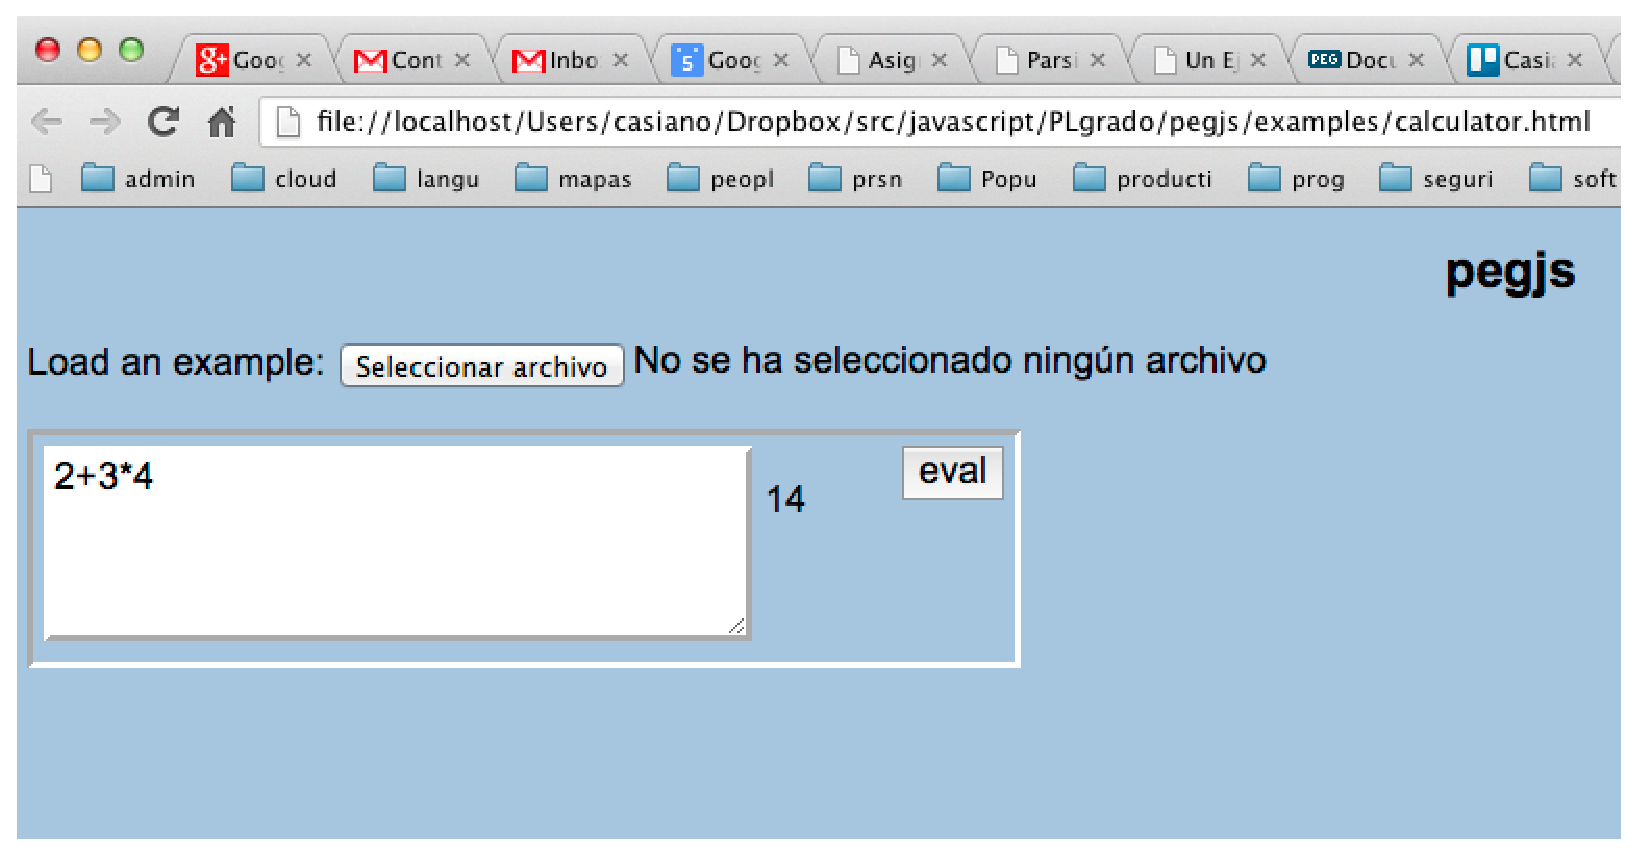
\epsfig{file=chapter_descendente/pegjs.eps, width=12cm}}
\caption{pegjs en la web}
\label{fig:pegjs}
\end{figure}
\end{center}
\end{latexonly}


\section{Eliminación de la Recursividad por la Izquierda en PEGs}

\subsection{Eliminación Usando Operadores de Repetición}
\parrafo{Donde}

\begin{itemize}
\item
\begin{verbatim}
[~/srcPLgrado/pegjs-coffee-plugin/examples(master)]$ pwd -P
/Users/casiano/local/src/javascript/PLgrado/pegjs-coffee-plugin/examples
\end{verbatim}
\item
\begin{verbatim}
[~/srcPLgrado/pegjs-coffee-plugin/examples(master)]$ git remote -v
dignifiedquire  git@github.com:Dignifiedquire/pegjs-coffee-plugin.git (fetch)
dignifiedquire  git@github.com:Dignifiedquire/pegjs-coffee-plugin.git (push)
origin  git@github.com:crguezl/pegjs-coffee-plugin.git (fetch)
origin  git@github.com:crguezl/pegjs-coffee-plugin.git (push)
\end{verbatim}
\item
\htmladdnormallink{https://github.com/crguezl/pegjs-coffee-plugin/tree/master/examples}{https://github.com/crguezl/pegjs-coffee-plugin/tree/master/examples}
\end{itemize}


\parrafo{Un Esquema de Traducción Recursivo por la Izquierda}
Consideremos el siguiente esquema de traducción implementado en \jison{}:

\begin{verbatim}
[~/srcPLgrado/pegjs-coffee-plugin/examples(master)]$ cat leftrec.jison 
/*
Exercise: Find a PEG equivalent to the following left-recursive
grammar:
*/
%lex
%%

\s+               { /* skip whitespace */ }
y                 { return 'y';}
.                 { return 'x';}

/lex

%{
  do_y = function(y)   { console.log("A -> 'y'   do_y("+y+")"); return y; }
  do_x = function(a, x){ console.log("A -> A 'x' do_x("+a+", "+x+")"); return a+x; }
%}

%%
A : A 'x' { $$ = do_x($1, $2); } 
  | 'y'   { $$ = do_y($1); }
;
\end{verbatim}

\begin{verbatim}
[~/srcPLgrado/pegjs-coffee-plugin/examples(master)]$ jison leftrec.jison 
[~/srcPLgrado/pegjs-coffee-plugin/examples(master)]$ ls -ltr leftrec.j*
-rw-r--r--  1 casiano  staff    441 18 mar 20:22 leftrec.jison
-rw-r--r--  1 casiano  staff  20464 18 mar 20:34 leftrec.js
\end{verbatim}

\begin{verbatim}
[~/srcPLgrado/pegjs-coffee-plugin/examples(master)]$ cat main_leftrec.js 
var parser = require('./leftrec');
input = "y x x x";
var r = parser.parse(input);
\end{verbatim}

\begin{verbatim}
[~/srcPLgrado/pegjs-coffee-plugin/examples(master)]$ node main_leftrec.js 
A -> 'y'   do_y(y)
A -> A 'x' do_x(y, x)
A -> A 'x' do_x(yx, x)
A -> A 'x' do_x(yxx, x)
\end{verbatim}

\parrafo{Métodología}

Es posible modificar la gramática para eliminar la recursión por 
la izquierda. En este apartado nos limitaremos al caso de recursión 
por la izquierda directa. 
La generalización al caso de recursión por la izquierda no-directa
se reduce a la iteración de la solución propuesta 
para el caso directo.

Consideremos una variable $A$ con dos producciones:

\vspace{0.25cm}
\begin{center}
$A   \rightarrow A \alpha |\ \beta$  
\end{center}

\noindent donde $\alpha, \beta \in (V \cup \Sigma)^*$ no comienzan por $A$.
Estas dos producciones pueden ser sustituidas por:

\vspace{0.25cm}
\begin{center}
$A   \rightarrow \beta \alpha * $ 
\end{center}

\noindent
eliminando así la recursión por la izquierda.


\parrafo{Solución}
\begin{verbatim}
[~/pegjs-coffee-remove-left(master)]$ cat -n remove_left_recursive.pegjs 
     1  /*
     2  
     3  Exercise: Find a PEG equivalent to the following left-recursive
     4  grammar:
     5  
     6  A : A 'x' { $$ = do_x($1, $2); } | 'y' { $$ = do_y($1); }
     7  
     8  */
     9  
    10  {
    11    @do_y = (y)   -> console.log("do_y(#{y})"); y
    12    @do_x = (a, x)-> console.log("do_x(#{a}, #{x})"); a+x
    13  }
    14  
    15  A = y:'y' xs:('x'*) 
    16       {
    17          a = @do_y(y)
    18          for x in xs
    19            a = @do_x(a, x)
    20          a
    21       }
\end{verbatim}

\begin{verbatim}
[~/pegjs-coffee-remove-left(master)]$ pegjs --plugin pegjs-coffee-plugin remove_left_recursive.pegjs 
[~/pegjs-coffee-remove-left(master)]$ ls -ltr | tail -1
-rw-rw-r--  1 casiano  staff   8919  3 jun 10:42 remove_left_recursive.js
\end{verbatim}

\begin{verbatim}
[~/pegjs-coffee-remove-left(master)]$ cat use_remove_left.coffee 
PEG = require("./remove_left_recursive.js")
inputs = [
           "yxx"
           "y"
           "yxxx"
         ]

for input in inputs 
  console.log("input = #{input}")
  r = PEG.parse input
  console.log("result = #{r}\n")
\end{verbatim}


\begin{verbatim}
[~/pegjs-coffee-remove-left(master)]$ coffee use_remove_left.coffee 
input = yxx
do_y(y)
do_x(y, x)
do_x(yx, x)
result = yxx

input = y
do_y(y)
result = y

input = yxxx
do_y(y)
do_x(y, x)
do_x(yx, x)
do_x(yxx, x)
result = yxxx
\end{verbatim}

\subsection{Eliminado la Recursividad por la Izquierda en la Calculadora Usando Operadores de Repetición}
\begin{verbatim}
[~/Dropbox/src/javascript/PLgrado/pegjs/examples(master)]$ cat simple.pegjs 
/* From the Wikipedia
Value   ← [0-9]+ / '(' Expr ')'
Product ← Value (('*' / '/') Value)*
Sum     ← Product (('+' / '-') Product)*
Expr    ← Sum
*/
{ 
  function reduce(left, right) {
    var sum = left;
    // console.log("sum = "+sum);
    for(var i = 0; i < right.length;i++) {
      var t = right[i];
      var op = t[0];
      var num = t[1];
      switch(op) {
        case '+' : sum += num; break;
        case '-' : sum -= num; break;
        case '*' : sum *= num; break;
        case '/' : sum /= num; break;
        default : console.log("Error! "+op);
      }
      // console.log("sum = "+sum);
    }
    return sum;
  }
}

sum   = left:product right:($[+-] product)* { return reduce(left, right); }
product = left:value right:($[*/] value)*   { return reduce(left, right); }
value   = number:$[0-9]+                    { return parseInt(number,10); }
        / '(' sum:sum ')'                   { return sum; }
\end{verbatim}

Es posible especificar mediante llaves  un código 
que este disponible dentro de las acciones semánticas.


Ejecución:
\begin{verbatim}
[~/pegjs/examples(master)]$ cat use_simple.js 
var PEG = require("./simple.js");
var r = PEG.parse("2-3-4");
console.log(r);

[~/pegjs/examples(master)]$ node use_simple.js 
-5
\end{verbatim}
Veamos otra ejecución:
\begin{verbatim}
[~/Dropbox/src/javascript/PLgrado/pegjs/examples(master)]$ cat use_simple.js 
var PEG = require("./simple.js");
var r = PEG.parse("2+3*(2+1)-10/2");
console.log(r);

[~/Dropbox/src/javascript/PLgrado/pegjs/examples(master)]$ ../bin/pegjs simple.pegjs 
[~/Dropbox/src/javascript/PLgrado/pegjs/examples(master)]$ node use_simple.js 
6
\end{verbatim}

\subsection{Eliminación Usando Predicados Semánticos: Sólo Sintáxis}
\label{subsection:eliminaleftrec}
La sección anterior da una forma sencilla de resolver el problema respetando la semántica.
Si no se dispone de operadores de repetición la cosa se vuelve mas complicada.
Las siguientes secciones muestran una solución para transformar un esquema de traducción
recursivo por la izquierda en otro no recursivo por la izquierda
respetando el orden en el que se ejecutan las acciones semánticas.
Por último se ilustra como se puede aplicar esta técnica en \verb|pegjs| (aunque 
obviamente es mucho mejor
usar la ilustrada anteriormente).

Es posible modificar la gramática para eliminar la recursión por 
la izquierda. En este apartado nos limitaremos al caso de recursión 
por la izquierda directa. 
La generalización al caso de recursión por la izquierda no-directa
se reduce a la iteración de la solución propuesta 
para el caso directo.

Consideremos una variable $A$ con dos producciones:

\vspace{0.25cm}
\begin{center}
$A   \rightarrow A \alpha |\ \beta$  
\end{center}

\noindent donde $\alpha, \beta \in (V \cup \Sigma)^*$ no comienzan por $A$.
Estas dos producciones pueden ser sustituidas por:

\vspace{0.25cm}
\begin{center}
\begin{tabular}{l}
$A   \rightarrow \beta R$\\
$R   \rightarrow  \alpha R\ |\ \epsilon$
\end{tabular}
\end{center}

\noindent
eliminando así la recursión por la izquierda.

\begin{definition}
La producción $R   \rightarrow  \alpha R$ se dice \cei{recursiva por la derecha}.
\end{definition}

Las producciones recursivas por la derecha dan lugar a árboles
que se hunden hacia la derecha. Es mas difícil traducir desde esta clase
de árboles operadores como el menos, que son asociativos a izquierdas.

\begin{exercise}
Elimine la recursión por la izquierda de la gramática 

\vspace{0.5cm}
\begin{tabular}{l}
$expr   \rightarrow expr  -  NUM$  \\
$expr   \rightarrow NUM$            
\end{tabular}
\vspace{0.5cm}

\end{exercise}


\subsection{Eliminación de la Recursión por la Izquierda Incluyendo la Semántica}
\label{subsection:eliminarecesquem}
La eliminación de la recursión por la izquierda es sólo un paso: debe 
ser extendida a esquemas de traducción, 
de manera que no sólo se preserve el lenguaje
sino la secuencia de acciones. Supongamos que tenemos un esquema de
traducción de la forma:

\vspace{0.25cm}
\begin{tabular}{ll}
$A   \rightarrow A \alpha$  & \verb|{ alpha_action }|\\
$A   \rightarrow A \beta$   & \verb|{ beta_action }|\\
$A   \rightarrow \gamma$    & \verb|{ gamma_action }|
\end{tabular}
\vspace{0.25cm}

\noindent para una sentencia como $\gamma \beta \alpha$ la secuencia de
acciones será: 

\begin{center}
\verb|gamma_action  beta_action alpha_action|
\end{center}

¿Cómo construir un esquema de traducción para la gramática resultante
de eliminar la recursión por la izquierda que ejecute las acciones
asociadas en el mismo orden?. Supongamos para simplificar,
que las acciones no dependen
de atributos ni computan atributos, sino que actúan sobre
variables globales. En tal caso, la siguiente
ubicación de las acciones da lugar a que se ejecuten en el mismo
orden:

\vspace{0.25cm}
\begin{center}
\begin{tabular}{l}
$A   \rightarrow \gamma$ \verb|{ gamma_action }| $R$\\
$R   \rightarrow \beta$ \verb| { beta_action }| $R$\\
$R   \rightarrow \alpha$ \verb| { alpha_action }| $R$\\
$R   \rightarrow \epsilon$  
\end{tabular}
\end{center}

Si hay atributos en juego, la estrategia para construir un
esquema de traducción equivalente para la gramática resultante
de eliminar la recursividad por la izquierda se complica.
Consideremos de nuevo el esquema de traducción de infijo a
postfijo de expresiones aritméticas de restas:

\vspace{0.5cm}
\begin{center}
\begin{tabular}{ll}
$expr   \rightarrow expr_1  -  NUM$  & \verb|{ $expr{T} = $expr[1]{T}+" "+$NUM{VAL}+" - "}| \\
$expr   \rightarrow NUM$             & \verb|{ $expr{T} = $NUM{VAL} }|
\end{tabular}
\vspace{0.5cm}
\end{center}

En este caso introducimos un atributo \verb|H| para los nodos de la clase
$r$ el cuál 
acumula la traducción a postfijo hasta el momento. Observe como
este atributo se computa en un nodo $r$ a partir del
correspondiente atributo del el padre y/o de los hermanos del nodo:

\vspace{0.5cm}
\begin{center}
\noindent
$expr   \rightarrow NUM$ \verb|{ $r{H} = $NUM{VAL} }|  $r$ \verb|{ $expr{T} = $r{T} }| \\
$r   \rightarrow - NUM$ \verb|{ $r_1{H} = $r{H}+" "+$NUM{VAL}." - " }| $r_1$ \verb|{ $r{T} = $r_1{T} }|\\
$r \rightarrow \epsilon$ \verb|{ $r{T} = $r{H} }|
\end{center}
\vspace{0.5cm}

El atributo \verb|H| es un ejemplo de atributo heredado.

\subsection{Atributos Heredados y PEGJS}

PegJS no permite acciones intermedias aunque si predicados semánticos. 
Tampoco se puede acceder al atributo 
de la parte izquierda.
Por eso, a la hora de implantar la solución anterior debemos introducir 
predicados semánticos.

Además nos obliga a usar variables visibles por todas las reglas semánticas para emular el acceso
a los atributos de la parte izquierda de una regla de producción.

El siguiente ejemplo ilustra como eliminar la recursión por la izquierda respetando la asociatividad de la operación de diferencia:

\begin{verbatim}
[~/srcPLgrado/pegjs/examples(master)]$ cat inherited2.pegjs 
{
  var h = 0, number = 0;
}

e = NUMBER &{ h = number; return true; } r { return h; }

r = '-' NUMBER &{ h -= number; return true; } r  { return h; } / /* empty */

NUMBER = _ digits:$[0-9]+ _  { number = parseInt(digits, 10); return number; }

_ = $[ \t\n\r]*
\end{verbatim}
Aquí \verb|h| - aún cuando se trata de una variable compartida - 
es usado como si fuera un atributo de los símbolos del PEG. Un tal atributo se 
denomina \cei{heredado}.

Este es el código para usar el PEG anterior:
\begin{verbatim}
[~/srcPLgrado/pegjs/examples(master)]$ cat use_inherited2.js 
var PEG = require("./inherited2.js");
var input = process.argv[2] || "5-1-2";
var r = PEG.parse(input);
console.log(r);
\end{verbatim}

Al ejecutarlo obtenemos:
\begin{verbatim}
[~/srcPLgrado/pegjs/examples(master)]$ pegjs inherited2.pegjs 
[~/srcPLgrado/pegjs/examples(master)]$ node use_inherited2.js 4-3-1
0
[~/srcPLgrado/pegjs/examples(master)]$ node use_inherited2.js 7-1-2
4
\end{verbatim}

\subsection{Eliminado la Recursividad por la Izquierda en la Calculadora Usando Predicados Semánticos}
En este ejemplo ilustramos como podemos insertar predicados semánticos entre los operadores de 
repetición para obtener la semántica deseada:
\begin{verbatim}
[~/srcPLgrado/pegjs/examples(master)]$ cat simple2.pegjs 
{
  var sum = 0;
  var initsum = function(first) { 
    sum = first; 
    return true; 
  };
  var add = function(op, p) {
    switch(op) {
        case '+':
            sum += p; 
            break;
        case '-':
            sum -= p; 
            break;
        default:
            error('"+" or "-" expected');
    }
    return true;
  };
}

sum     = first:value &{ return initsum(first); } (op:[+-] product:value & { return add(op, product); })* { return sum; } 
value   = number:$[0-9]+                     { return parseInt(number,10); }
        / '(' sum:sum ')'                    { return sum; }
\end{verbatim}
El primer predicado \verb|first:value &{ return initsum(first); }| inicializa la suma.
A continuación y aprovechando el cierre \verb|*| se ejecuta en bucle el segundo predicado
\verb|(op:[+-] product:value & { return add(op, product); })| que va acumulando el resultado.
La acción semántica final se limita a retornar el resultado acumulado.
\begin{verbatim}
[~/srcPLgrado/pegjs/examples(master)]$ cat use_simple2.js
var PEG = require("./simple2.js");
var input = process.argv[2] || "5-1-2";
var r = PEG.parse(input);
console.log(r);
\end{verbatim}

\begin{verbatim}
[~/srcPLgrado/pegjs/examples(master)]$ pegjs simple2.pegjs 
[~/srcPLgrado/pegjs/examples(master)]$ node use_simple2.js 3-1-5
-3
\end{verbatim}

\parrafo{Encapsulando la Solución}

La variable \verb|sum| es excesivamente visible. Podemos encapsularla un poco mas:

\begin{verbatim}
[~/srcPLgrado/pegjs/examples(master)]$ cat simple3.pegjs 
{
  var sum = (function() {
    var sum = 0;
    var get = function() { return sum; };
    var set = function(first) { 
      sum = first; 
      return true; 
    };
    var add = function(op, p) {
      switch(op) {
          case '+':
              sum += p; 
              break;
          case '-':
              sum -= p; 
              break;
          default:
              error('"+" or "-" expected');
      }
      return true;
    };
    return {s: set, a: add, g: get };
  })();
}

sum     = first:value &{ return sum.s(first); } (op:[+-] product:value & { return sum.a(op, product); })* { return sum.g(); } 
value   = number:$[0-9]+                     { return parseInt(number,10); }
        / '(' sum:sum ')'                    { return sum; }
\end{verbatim}

\begin{verbatim}
[~/srcPLgrado/pegjs/examples(master)]$ cat use_simple3.js 
var PEG = require("./simple3.js");
var input = process.argv[2] || "5-1-2";
var r = PEG.parse(input);
console.log(r);
\end{verbatim}

\begin{verbatim}
[~/srcPLgrado/pegjs/examples(master)]$ pegjs simple3.pegjs 
[~/srcPLgrado/pegjs/examples(master)]$ node use_simple3.js 4-1-1
2
[~/srcPLgrado/pegjs/examples(master)]$ node use_simple3.js 4-1-4
-1
\end{verbatim}

\section{Reconocimiento de Lenguajes con PEGjs}

\subsection{PEGs versus Gramáticas}
\label{subsection:pegvsgrammars}

Una gramática y un PEG con las mismas reglas no definen el mismo lenguaje.
Véase este ejemplo:
\begin{verbatim}
[~/srcPLgrado/pegjs/examples(master)]$ cat grammarvspeg.coffee 
#!/usr/bin/env coffee
PEG = require 'pegjs'
coffee = require 'pegjs-coffee-plugin'
grammar = """
a =  b 'c'           
b = 'b' / 'b' 'a'   
"""
parser = PEG.buildParser grammar, plugins: [coffee]
r = parser.parse "bc"
console.log("r = #{r}")
r = parser.parse "bac"
console.log("r = #{r}")
[~/srcPLgrado/pegjs/examples(master)]$ coffee grammarvspeg.coffee 
r = b,c
SyntaxError: Expected "c" but "a" found.
\end{verbatim}

Obsérvese que la correspondiente gramática genera el lenguaje:
\begin{verbatim}
{ 'bc', 'bac' }
\end{verbatim}
Mientras que el PEG acepta el lenguaje \verb|'bc'|.

\subsection{\red{Dangling else}: Asociando un else con su if mas cercano}

The dangling else is a problem in computer programming in which an
optional \verb|else clause| in an \verb|If–then(–else)| statement results in nested
conditionals being ambiguous. 

Formally, the reference context-free
grammar of the language is ambiguous, meaning there is more than one
correct parse tree.

In many programming languages one may write conditionally executed code
in two forms: 

the \verb|if-then| form, and the \verb|if-then-else| form – the 
\verb|else|
clause is optional:
\begin{verbatim}
              if a then s
              if a then s1 else s2
\end{verbatim}

This gives rise to an ambiguity in interpretation when there are nested
statements, specifically whenever an \verb|if-then| form appears as \verb|s1|
in an \verb|if-then-else| form:
\begin{verbatim}
              if a then if b then s else s2
\end{verbatim}
In this example, \verb|s| is unambiguously executed when \verb|a| is
\verb|true| and \verb|b| is \verb|true|, but one may interpret \verb|s2|
as being executed when \verb|a| is \verb|false| 
\begin{itemize}
\item
(thus attaching the
\verb|else| to the first \verb|if|) or when 
\item
\verb|a| is \verb|true|
and \verb|b| is \verb|false| (thus attaching the \verb|else| to the
second \verb|if|). 
\end{itemize}
In other words, one may see the previous statement
as either of the following expressions:
\begin{verbatim}
if a then (if b then s) else s2
\end{verbatim}
      or
\begin{verbatim}
if a then (if b then s else s2)
\end{verbatim}

This is a problem that often comes up in compiler construction,
especially scannerless parsing. 

The convention when dealing with
the dangling \verb|else| is to attach the \verb|else| to the nearby
\verb|if| statement.

Programming languages like Pascal and C follow this
convention, so there is no ambiguity in the semantics of the language,
though the use of a parser generator may lead to ambiguous grammars. 
In
these cases \red{alternative grouping is accomplished by explicit blocks},
such as \verb|begin...end| in Pascal and \verb|{...}| in C.

Here follows a solution in PEG.js:

\parrafo{danglingelse.pegjs}
\begin{verbatim}
$ cat danglingelse.pegjs 
/*
S ← 'if' C 'then' S 'else' S / 'if' C 'then' S
*/

S =   if C:C then S1:S else S2:S { return [ 'ifthenelse', C, S1, S2 ]; }
    / if C:C then S:S            { return [ 'ifthen', C, S]; }
    / O                          { return 'O'; }
_ = ' '*
C = _'c'_                        { return 'c'; }
O = _'o'_                        { return 'o'; }
else = _'else'_                 
if = _'if'_
then = _'then'_
\end{verbatim}

\parrafo{use\_danglingelse.js}

\begin{verbatim}
$ cat use_danglingelse.js 
var PEG = require("./danglingelse.js");
var r = PEG.parse("if c then if c then o else o");
console.log(r);
\end{verbatim}


\parrafo{Ejecución}
\begin{verbatim}
$ ../bin/pegjs danglingelse.pegjs 
$ node use_danglingelse.js 
[ 'ifthen', 'c', [ 'ifthenelse', 'c', 'O', 'O' ] ]
\end{verbatim}

\parrafo{Donde}

\begin{itemize}
\item
\begin{verbatim}
[~/srcPLgrado/pegjs/examples(master)]$ pwd -P
/Users/casiano/local/src/javascript/PLgrado/pegjs/examples
\end{verbatim}

\item
\begin{verbatim}
[~/srcPLgrado/pegjs/examples(master)]$ git remote -v
dmajda  https://github.com/dmajda/pegjs.git (fetch)
dmajda  https://github.com/dmajda/pegjs.git (push)
origin  git@github.com:crguezl/pegjs.git (fetch)
origin  git@github.com:crguezl/pegjs.git (push)
\end{verbatim}
\item
\htmladdnormallink{https://github.com/crguezl/pegjs/tree/master/examples}{https://github.com/crguezl/pegjs/tree/master/examples}
\end{itemize}

\parrafo{Invirtiendo el orden de las Alternativas}

Si invertimos el orden de las alternativas:
\begin{verbatim}
[~/srcPLgrado/pegjs/examples(master)]$ cat danglingelse2.pegjs 
/*
S ← 'if' C 'then' S 'else' S / 'if' C 'then' S
*/

S =   if C:C then S:S            { return [ 'ifthen', C, S]; }
    / if C:C then S1:S else S2:S { return [ 'ifthenelse', C, S1, S2 ]; }
    / O                          { return 'O'; }
_ = ' '*
C = _'c'_                        { return 'c'; }
O = _'o'_                        { return 'o'; }
else = _'else'_                 
if = _'if'_
then = _'then'_
\end{verbatim}
el lenguaje reconocido cambia (vease el ejemplo
en  la sección
\ref{subsection:pegvsgrammars}):
\begin{verbatim}
[~/srcPLgrado/pegjs/examples(master)]$ pegjs danglingelse2.pegjs 
[~/srcPLgrado/pegjs/examples(master)]$ cat use_danglingelse2.js 
var PEG = require("./danglingelse2.js");
var r = PEG.parse("if c then if c then o else o");
console.log(JSON.stringify(r));

[~/srcPLgrado/pegjs/examples(master)]$ node use_danglingelse2.js 

/Users/casiano/local/src/javascript/PLgrado/pegjs/examples/danglingelse2.js:513
      throw peg$buildException(null, peg$maxFailExpected, peg$maxFailPos);
            ^
SyntaxError: Expected " " or end of input but "e" found.
\end{verbatim}

\subsection{Not Predicate: Comentarios Anidados}
The following recursive \pegjs{}
program  matches Pascal-style nested comment syntax:
\begin{verbatim}
(* which can (* nest *) like this *)
\end{verbatim}

\parrafo{Pascal\_comments.pegjs}
\begin{verbatim}
[~/srcPLgrado/pegjs/examples(master)]$ cat pascal_comments.pegjs 
/* Pascal nested comments */

P     =   prog:N+                       { return prog; }
N     =   chars:$(!Begin .)+            { return chars;}
        / C
C     = Begin chars:$T* End             { return "C: "+chars; }
T     =   C 
        / (!Begin !End char:.)          { return char;}
Begin = '(*'
End   = '*)'
\end{verbatim}

\parrafo{use\_pascal\_comments.js}
\begin{verbatim}
$ cat use_pascal_comments.js 
var PEG = require("./pascal_comments.js");
var r = PEG.parse(
  "not bla bla (* pascal (* nested *) comment *)"+
  " pum pum (* another comment *)");
console.log(r);
\end{verbatim}

\parrafo{Ejecución}
\begin{verbatim}
$ ../bin/pegjs pascal_comments.pegjs 
$ node use_pascal_comments.js 
[ 'not bla bla ',
  ' pascal  nested  comment ',
  ' pum pum ',
  ' another comment ' ]
\end{verbatim}

\parrafo{Donde}

\begin{itemize}
\item
\begin{verbatim}
[~/srcPLgrado/pegjs/examples(master)]$ pwd -P
/Users/casiano/local/src/javascript/PLgrado/pegjs/examples
\end{verbatim}

\item
\begin{verbatim}
[~/srcPLgrado/pegjs/examples(master)]$ git remote -v
dmajda  https://github.com/dmajda/pegjs.git (fetch)
dmajda  https://github.com/dmajda/pegjs.git (push)
origin  git@github.com:crguezl/pegjs.git (fetch)
origin  git@github.com:crguezl/pegjs.git (push)
\end{verbatim}
\item
\htmladdnormallink{https://github.com/crguezl/pegjs/tree/master/examples}{https://github.com/crguezl/pegjs/tree/master/examples}
\end{itemize}

\subsection{Un Lenguaje Dependiente del Contexto}

El lenguaje $\{ a^n b^n c^n / n \in \mathcal{N} \}$ no puede ser 
expresado mediante una gramática independiente del contexto.
 
\begin{verbatim}
[~/srcPLgrado/pegjs/examples(master)]$ cat anbncn.pegjs 
/*
  The following parsing expression grammar describes the classic 
  non-context-free language : 
               { a^nb^nc^n / n >= 1 }
*/

S = &(A 'c') 'a'+ B:B !.  { return B; }
A = 'a' A:A? 'b' { if (A) { return A+1; } else return 1; }
B = 'b' B:B? 'c' { if (B) { return B+1; } else return 1; }
\end{verbatim}

Este ejemplo puede ser obtenido desde GitHub:
\begin{verbatim}
[~/Dropbox/src/javascript/PLgrado/pegjs/examples(master)]$ git remote -v
dmajda  https://github.com/dmajda/pegjs.git (fetch)
dmajda  https://github.com/dmajda/pegjs.git (push)
origin  git@github.com:crguezl/pegjs.git (fetch)
origin  git@github.com:crguezl/pegjs.git (push)
\end{verbatim}

Veamos un ejemplo de uso:
\begin{verbatim}
[~/srcPLgrado/pegjs/examples(master)]$ cat use_anbncn.js 
#!/usr/bin/env node
var PEG = require("./anbncn.js");

if (process.argv.length > 2) {
  try {
    var r = PEG.parse(process.argv[2]);
    console.log("ok "+JSON.stringify(r));
  }
  catch (e) {
    console.log("Grr...."+e);
  }
  process.exit(0);
}
var inputs = ["aabbcc", 
              "aabbc",     // error
              "aaabbbccc",
              "aaaabbbccc"  // not accepted
             ];

for(var i = 0; i < inputs.length; i++) {
  var input = inputs[i];
  try {
    var r = PEG.parse(input);
    console.log("ok "+JSON.stringify(r));
  }
  catch (e) {
    console.log("Grr...."+e);
  }
}
\end{verbatim}

Ejecución:
\begin{verbatim}
[~/srcPLgrado/pegjs/examples(master)]$ node use_anbncn.js
ok 2
Grr....SyntaxError: Expected "c" but end of input found.
ok 3
Grr....SyntaxError: Expected undefined but "a" found.
\end{verbatim}

\sectionpractica{Analizador de PL0 Usando PEG.js}
Reescriba el analizador sintáctico del lenguaje PL0 
realizado en la práctica 
\ref{practica:pl0}
usando \pegjs{}.

\sectionpractica{Analizador de PL0 Ampliado Usando PEG.js}
\label{practica:pl0ampliado}
Reescriba el analizador sintáctico del lenguaje PL0 
realizado en la práctica 
\ref{practica:pl0}
usando \pegjs{}.

\parrafo{Donde}

\begin{itemize}
\item
\htmladdnormallink{Repositorio en GitHub}{https://github.com/crguezl/pegjscalc}
\item
\htmladdnormallink{Despliegue en Heroku}{http://pegjspl0.herokuapp.com/}
\item
\begin{verbatim}
[~/srcPLgrado/pegjscalc(master)]$ pwd -P
/Users/casiano/local/src/javascript/PLgrado/pegjscalc
\end{verbatim}
\item
\begin{verbatim}
[~/srcPLgrado/pegjscalc(master)]$ git remote -v
heroku  git@heroku.com:pegjspl0.git (fetch)
heroku  git@heroku.com:pegjspl0.git (push)
origin  git@github.com:crguezl/pegjscalc.git (fetch)
origin  git@github.com:crguezl/pegjscalc.git (push)
\end{verbatim}
\end{itemize}

\parrafo{Tareas}
\begin{itemize}
\item
Modifique \verb|block| y \verb|statement| para que los 
\verb|procedure| reciban argumentos y las llamadas 
a procedimiento puedan pasar argumentos.
Añada \verb|if ... then ... else ...|.
\item Actualice la documentación de la gramática para que refleje la gramática ampliada
\item
Limite el número de programas que se pueden salvar a un número prefijado, por ejemplo 10. Si se intenta salvar uno se suprime uno al azar y se guarda el nuevo.
\item
Las pruebas deben comprobar que la asociatividad a izquierdas funciona bien
y probar todos los constructos del lenguaje así como alguna situación de error
\end{itemize}

\parrafo{Referencias para esta Práctica}
\begin{itemize}
\item Véase el capítulo {\it Heroku} \ref{chapter:heroku}
\item
\htmladdnormallink{Heroku Postgres}{https://devcenter.heroku.com/articles/heroku-postgresql}
\item Véase el capítulo {\it DataMapper} \ref{chapter:datamapper}
\end{itemize}

\sectionpractica{Ambiguedad en C++}
This lab illustrates a problem 
that arises in C++.
The C++ syntax does not disambiguate between expression
statements (\verb|stmt|) and declaration statements (\verb|decl|). 
The ambiguity arises when an expression
statement has a function-style cast as its left-most subexpression.
Since C does not support function-style casts, this ambiguity does not occur
in C programs.
For example, the phrase 

\verb|int (x) = y+z;| 

parses as either a \texttt{decl} or a \texttt{stmt}.

The disambiguation rule used in C++ is that {\it
if the statement can be interpreted both as a declaration and
as an expression, the statement is interpreted as a declaration statement.
}

The following examples  disambiguate into {\it expression} statements when the
potential {\it declarator} is followed by an operator different from equal 
or semicolon (\texttt{type\_spec} stands for a type specifier):

\begin{center}
\begin{tabular}{|p{3.5cm}|p{4.5cm}|}
\hline
expr  & dec\\
\hline
\begin{verbatim}
type_spec(i)++;      
type_spec(i,3)<<d;  
type_spec(i)->l=24;
\end{verbatim}
&
\begin{verbatim}
type_spec(*i)(int); 
type_spec(j)[5];   
type_spec(m) = { 1, 2 }; 
type_spec(a);              
type_spec(*b)();          
type_spec(c)=23;         
type_spec(d),e,f,g=0;   
type_spec(h)(e,3);     
\end{verbatim}\\
\hline
\end{tabular}
\end{center}

Regarding to this problem, Bjarne Stroustrup remarks:
\begin{quote}
\begin{it}
 Consider analyzing a statement consisting of
a sequence of tokens as follows:
\begin{verbatim}
              type_spec (dec_or_exp) tail
\end{verbatim}
Here \verb|dec_or_exp| must be a declarator, an expression, 
or both for the statement to be legal. This implies that \verb|tail|
must be a semicolon, something that can follow a 
parenthesized declarator or something that can follow
a parenthesized expression, that is, an initializer, \verb|const|,
\verb|volatile|, \verb|(|, \verb|[|, or a postfix or infix operator.
The general cases cannot be resolved without backtracking, nested grammars
or similar advanced parsing strategies. In particular,
the lookahead needed to disambiguate this case is not limited.
\end{it}
\end{quote}

The following grammar 
depicts 
an oversimplified version of the C++ ambiguity:

\begin{verbatim}
$ cat CplusplusNested.y 
%token ID INT NUM

%right '='
%left '+'

%%
prog:
    /* empty */
  | prog stmt
;

stmt: 
    expr ';' 
  | decl    
;

expr:
    ID 
  | NUM
  | INT '(' expr ')' /* typecast */ 
  | expr '+' expr
  | expr '=' expr
;

decl:
    INT declarator ';'
  | INT declarator '=' expr ';'
;

declarator:
    ID 
  | '(' declarator ')'
;

%%
\end{verbatim}

Escriba un programa PegJS en CoffeeScript que distinga correctamente entre declaraciones
y sentencias. Este es un ejemplo de un programa que usa una solución al problema:
\begin{verbatim}
[~/Dropbox/src/javascript/PLgrado/pegjs-coffee-plugin/examples(master)]$ cat use_cplusplus.coffee 
PEG = require("./cplusplus.js")
input = "int (a); int c = int (b);"

r = PEG.parse(input)
console.log("input = '#{input}'\noutput="+JSON.stringify r)

input = "int b = 4+2  ;  "
r = PEG.parse(input)
console.log("input = '#{input}'\noutput="+JSON.stringify r)

input = "bum = caf = 4-1;\n"
r = PEG.parse(input)
console.log("input = '#{input}'\noutput="+JSON.stringify r)

input = "b2 = int(4);"
r = PEG.parse(input)
console.log("input = '#{input}'\noutput="+JSON.stringify r)

input = "int(4);"
r = PEG.parse(input)
console.log("input = '#{input}'\noutput="+JSON.stringify r)
\end{verbatim}
Y este un ejemplo de salida:
\begin{verbatim}
$ pegcoffee cplusplus.pegjs 
$ coffee use_cplusplus.coffee 
input = 'int (a); int c = int (b);'
output=["decl","decl"]
input = 'int b = 4+2  ;  '
output=["decl"]
input = 'bum = caf = 4-1;
'
output=["stmt"]
input = 'b2 = int(4);'
output=["stmt"]
input = 'int(4);'
output=["stmt"]
\end{verbatim}

\sectionpractica{Inventando un Lenguaje: Tortoise}

El objetivo de esta práctica es crear un lenguaje de programación 
imperativa sencillo de estilo \wikip{LOGO}{Logo\_programming\_language}.
Para ello lea el capítulo
\htmladdnormallink{Inventing a Language - Tortoise}{http://nathansuniversity.com/turtle.html}
del 
\htmladdnormallink{curso PL101: Create Your Own Programming Language}{http://nathansuniversity.com/turtle.html}
de 
\htmladdnormallink{Nathan Whitehead}{http://nathansjslessons.appspot.com/}.
Haga todos los ejercicios e implemente el lenguaje descrito.

Puede encontrar una solución a la práctica en GitHub en el repositorio
\htmladdnormallink{pl101}{https://github.com/dingram/pl101}
de 
\htmladdnormallink{Dave Ingram}{http://www.dmi.me.uk/blog/}. Usela como guía cuando se sienta desorientado.

\parrafo{Recursos}
\begin{itemize}
\item
\htmladdnormallink{Inventing a Language - Tortoise}{http://nathansuniversity.com/turtle.html}
por Nathan Whitehead
\item
Repositorio
\htmladdnormallink{dingram / pl101 en GitHub}{https://github.com/dingram/pl101}
con las soluciones a esta práctica. 

  \begin{itemize}
  \item Blog de \htmladdnormallink{dingram (Dave Ingram)}{http://www.dmi.me.uk/blog/}
  \end{itemize}
\item
Repositorio
\htmladdnormallink{PatrixCR / PL101 en GitHub}{https://github.com/PatrixCR/PL101}
con las soluciones a esta práctica. 

\item
Repositorio
\htmladdnormallink{Clinton N. Dreisbach/ PL101 en GitHub}{https://github.com/cndreisbach/PL101}
con contenidos del curso PL101

\item
\htmladdnormallink{Foro}{http://nathansuniversity.com/vanilla/discussion/79/lesson-6-inventing-a-language-for-turtle-graphics/p1}

\item Sobre Nathan Whitehead
  \begin{itemize}
  \item
  \htmladdnormallink{Nathan's Lessons}{http://nathansjslessons.appspot.com/}
\item
\htmladdnormallink{Nathan Whitehead en GitHub}{https://github.com/nwhitehead}
\item
\htmladdnormallink{Nathan in YouTube}{http://www.youtube.com/user/NathanWhitehead}
  \end{itemize}
\end{itemize}
